\chapter{Hardening a Hadoop Cluster}\label{chap:5}
In this chapter, we will cover:
\begin{itemize}
  \item Configuring service level authentication
  \item Configuring job authorization with ACL
  \item Securing Hadoop cluster with Kerberos
  \item Configuring web UI authentication
  \item Recovering from NameNode failure
  \item Configuring NameNode high availability
  \item Configuring HDFS federation
\end{itemize}

\section{Introduction}
The security of a Hadoop cluster is critical for its availability. Hardening a Hadoop cluster includes configuring access control over resources such as jobs, queues and various administrative services. We will introduce NameNode High Availability (HA) for the problem of single node failure. In the end, we will introduce Hadoop federation, which federates multiple machines to expand the capacity of a cluster.

\section{Configuring service level authentication}
The purpose of service level authentication (SLA) is to ensure that Hadoop users have the proper permission to access certain services. One use case of this configuration is to control a list of allowed users who can use the cluster. This is enforced with Access Control List (ACL) in Hadoop. In this recipe, we will list steps to configure SLA.

\subsection*{Getting ready}
Before getting started, we assume that our Hadoop cluster has been properly configured and all the daemons are running without any issues.
Login to the master node from the administrator machine with command:
ssh hduser@master

\subsection*{How to do it...}
Use the following steps to configure Hadoop SLA:

Enable SLA by opening file \verb|$HADOOP_HOME/conf/core-site.xml| and add or change the \verb|hadoop.property.authorization| to be true as shown in the following:
\lstset{style=bashstyle}
\begin{lstlisting}[language=XML]
<property>
  <name>hadoop.property.authorization</name>
  <value>true</name>
</property>
\end{lstlisting}

SLA of a Hadoop cluster is disabled by default.

Allow only specific users to submit jobs to the Hadoop cluster by adding or changing the following property in file \verb|$HADOOP_HOME/conf/hadoop-policy.xml|:
\lstset{style=bashstyle}
\begin{lstlisting}[language=XML]
<property>
  <name>security.job.submission.protocol.acl</name>
  <value>hduser hadoop</name>
</property>
\end{lstlisting}

This configuration only allows user hduser and group hadoop to submit jobs to the Hadoop cluster.

Allow only specific users and groups to talk to HDFS by opening file \verb|$HADOOP_HOME/conf/hadoop-policy.xml| and add the following property:
\lstset{style=bashstyle}
\begin{lstlisting}[language=XML]
<property>
  <name>security.client.protocol.acl</name>
  <value>hduser,hdadmin hadoop</name>
</property>
\end{lstlisting}

This configuration only allows users hduser and hdadmin and group hadoop to access HDFS.

Allows only specific DataNodes to communicate with the NameNode by changing the security.datanode.protocol.acl property in file \verb|$HADOOP_HOME/conf/hadoop-policy.xml| similar to the following:
\lstset{style=bashstyle}
\begin{lstlisting}[language=XML]
<property>
  <name>security.datanode.protocol.acl</name>
  <value>datanode</name>
</property>
\end{lstlisting}

This configuration only allows DataNodes running as users belonging to group datanode to communicate with the NameNode in the cluster.

Force the NameNode to reload the ACL configurations with command: \\
\verb|$ hadoop dfsadmin -refreshServiceAcl| \\

This command will force the reload the HDFS related ACLs from the policy file.

Force the JobTracker to reload the service ACL configurations with command: \\
\verb|$ hadoop mradmin -refreshServiceAcl|

\subsection*{How it works...}
The value of properties such as security.namenode.protocol.acl is a comma separated list of users and a comma separated list of groups. The users list and the groups list are separated by space. For example, the generic format of the value should be similar to the following: \\
\verb|<value>user1,user2,user3 group1,group2</value>|

\subsection*{There's more...}
Besides the three properties we mentioned in this recipe, a number of other ACL properties are available in Hadoop. The following table shows the meaning of these properties: \\
\begin{table}
  \centering
  \small
  \begin{tabular}{ll}
    \toprule
    Property & Service Description \\ \midrule
    security.client.protocol.acl & Clients access HDFS \\
    security.client.datanode.protocol.acl & Client to DataNode for block recovery \\
    security.inter.datanode.protocol.acl & DataNode to DataNode updating timestamps \\
    security.inter.tracker.protocol.acl & TaskTracker to JobTracker \\
    security.job.submission.protocol.acl & Client to JobTracker for job submission, querying and so on. \\
    security.task.umbilical.protocol.acl & For map and reduce tasks talk to TaskTracker. \\
    security.refresh.policy.protocol.acl & dfsadmin and mradmin to refresh ACL policies. \\ \bottomrule
  \end{tabular}
  \caption{ACL properties}\label{tbl:acl}
\end{table}

The default value of these properties is *, which means all entities can access the service or, in other words, SLA is disabled.
\subsection*{See also}
\begin{itemize}
  \item Configuring job authorization with ACLs
  \item \url{http://hadoop.apache.org/docs/r1.1.2/service_level_auth.html#Enable+Service+Level+Authorization}
\end{itemize}

Configuring job authorization with ACL
Hadoop provides two levels of job authorization: job level and queue level. When job authorization is enabled, the JobTracker will authenticate users who submit jobs to the cluster. Users' operations on jobs and queues will also be authenticated by the JobTracker. In this recipe, we will show steps to configure job authorization with ACLs.
\subsection*{Getting ready}
We assume that our Hadoop cluster has been properly configured without any problems.

Login to the master node from the administrator machine with command: \\
\verb|$ ssh hduser@master|
\subsection*{How to do it...}
Use the following steps to configure job authorization with ACLs:

Enable job ACL authorization by adding the following property to file \verb|$HADOOP_HOME/conf/mapred-site.xml|:
\lstset{style=bashstyle}
\begin{lstlisting}[language=XML]
<property>
  <name>mapred.acls.enabled</name>
  <value>true</name>
</property>
\end{lstlisting}
This property will enable both the queue ACL and the job ACL.

Configure to only allow specific users and groups to submit jobs by adding the following property to file \verb|$HADOOP_HOME/conf/mapred-queue-acls.xml|:
\lstset{style=bashstyle}
\begin{lstlisting}[language=XML]
<property>
  <name>mapred.queue.hdqueue.acl-submit-job</name>
  <value>hduser hadoop</name>
</property>
\end{lstlisting}

This configuration will only allow user hduser and group hadoop to submit jobs to queue hdqueue.

Configure to allow specific users and groups to manage jobs in a named queue by adding the following property to file \verb|$HADOOP_HOME/conf/mapred-queue-acls.xml|:
\lstset{style=bashstyle}
\begin{lstlisting}[language=XML]
<property>
  <name>mapred.queue.hdqueue.acl-administer-job</name>
  <value>hduser hadoop</name>
</property>
\end{lstlisting}

This configuration will only allow user hduser and group hadoop to administrate jobs to queue hdqueue.

Check the status of queue ACLs with command:
\lstset{style=bashstyle}
\begin{lstlisting}
$ hadoop queue -showacls
Queue acls for user :  hduser

Queue  Operations
=====================
default  submit-job,administer-jobs
hdqueue  submit-job,administer-jobs
\end{lstlisting}

Configure to allow only specific users and groups to view the status of a job by adding the following property to file \verb|$HADOOP_HOME/conf/mapred-queue-acls.xml|:
\lstset{style=bashstyle}
\begin{lstlisting}[language=XML]
<property>
  <name>mapreduce.job.acl-view-job</name>
  <value>hduser hadoop</name>
</property>
\end{lstlisting}

Different to queue level ACL, job level ACLs specifies access control for any submitted jobs, regardless of the queue a job has been submitted to.

Configure to allow only specific users and groups to modify a job by adding the following property to file \verb|$HADOOP_HOME/conf/mapred-queue-acls.xml|:
\lstset{style=bashstyle}
\begin{lstlisting}[language=XML]
<property>
  <name>mapreduce.job.acl-modify-job</name>
  <value>hduser hadoop</name>
</property>
\end{lstlisting}

Force the NameNode and the JobTracker to reload the ACL configurations with commands: \\
\verb|$ hadoop dfsadmin -refreshServiceAcl| \\
\verb|$ hadoop mradmin -refreshServiceAcl|

\subsection*{How it works...}
Similar to the SLA properties in the previous recipe, the value of properties such as mapred.queue.hdqueue.acl-submit-job is a comma separated list of users and a comma separated list of groups. The users list and the groups list are separated by space. For example,  the generic format of the value should be similar to the following: \\
\verb|<value>user1,user2,user3 group1,group2</value>|

\begin{info}
Note! \\
The job owner, the super user and the cluster administrators that the job was submitted to will always have right to view and modify a job.
\end{info}

Job view ACLs control the access of job status information including counters, diagnostic information, logs and job configuration and so on.

Job modification ACLs can overlap with queue level ACLs. When this happens, a user's operation will be granted if the user has been listed in either of these ACLs.
\subsection*{See also}
\begin{itemize}
  \item Configuring service level authentication
  \item \url{http://hadoop.apache.org/docs/r1.1.2/mapred_tutorial.html#Job+Authorization}
  \item \url{http://hadoop.apache.org/docs/r1.1.2/cluster_setup.html}
\end{itemize}

\section{Securing Hadoop cluster with Kerberos}
Recent Hadoop releases have added the security feature by integrating Kerberos into Hadoop. Kerberos is a network authentication protocol that provides strong authentication for client/server applications. Hadoop uses Kerberos to secure data from unexpected and unauthorized accesses. It achieves this by authenticating on the underlying Remote Procedure Calls (RPC). In this recipe, we will outline steps to configure Kerberos authentication for a Hadoop cluster.
\subsection*{Getting ready}
Kerberos was created by MIT. It was designed to provide strong authentication for client/server applications by using secret key cryptography. The Kerberos protocol requires that a client provide its identity to the server and vice versa. When their identities are proved by Kerberos, all of their following communication will be encrypted.

Before getting started, we assume that our Hadoop has been properly configured without any problems and all the Hadoop daemons are running without any issues.

Under our CentOS machine, use the following command to install the Kerberos packages: \\
\verb|$ sudo yum install krb5-libs, krb5-server, krb5-workstation|

After this, the kadmin and the kinit commands should be accessible from the command line.

If you are also using CentOS or other Red Had compatible operating systems, we need to install Java Cryptography Extension (JCE) Unlimited Strength Jurisdiction Policy Files, by downloading it from the following command: \url{http://www.oracle.com/technetwork/java/javase/downloads/index.html}

At the bottom of the web page, you should see options similar to Figure \ref{fig:jce}.
\begin{figure}[ht]
  \centering
  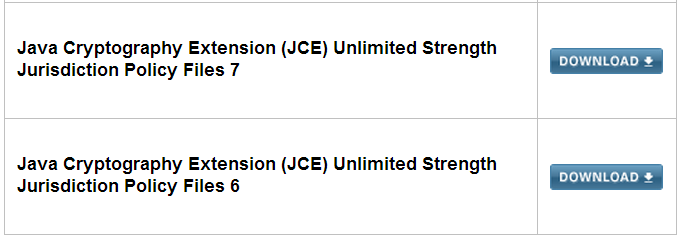
\includegraphics[width=.85\textwidth]{figs/5163os_05_01.png}
  \caption{Option of downloading JCE}\label{fig:jce}
\end{figure} 
Click the right download link based on your Java version, which we can get with the \verb|``java -version''| command.
\subsection*{How to do it...}
Use the following steps to configure Kerberos for a Hadoop cluster:

Start the Kerberos admin shell: \\
\verb|$ kadmin|

If your account does not have root access, you need to use the kadmin.local command:

Create the hduser principal with the following command in the kadmin shell: \\
\verb|$ addprinc -randkey hduser/master.hdcluster.com@HDREALM|

Create the HTTP principal for SPNEGO with command in the kadmin shell: \\
\verb|$ addprinc -randkey HTTP/master.hdcluster.com@HDREALM|

Create the keytab file that contains the hduser's and HTTP principal with: 
\lstset{style=bashstyle}
\begin{lstlisting}
$ xst -norandkey -k hduser.keytab hduser/master.hdcluster.com HTTP/master.hdcluster.com
\end{lstlisting}

Show available keytab file entries with:
\lstset{style=bashstyle}
\begin{lstlisting}
$ klist -e -k -t hduser.keytab
Keytab name: WRFILE:hduser.keytab
slot KVNO Principal
---- ---- ---------------------------------------------------------------
1    7    HTTP/master.hdcluster.com@HDREALM (DES cbc mode with CRC-32)
2    7    HTTP/master.hdcluster.com@HDREALM (Triple DES cbc mode with HMAC/sha1)
3    7    hduser/master.hdcluster.com@HDREALM (DES cbc mode with CRC-32)
4    7    hduser/master.hdcluster.com@HDREALM (Triple DES cbc mode with HMAC/sha1)
\end{lstlisting}

Move the keytab files to the Hadoop configuration directory with: \\
\verb|$ cp *.keytab $HADOOP_HOME/conf|

Change the owner of the hduser keytab file with:\\
\verb|$ sudo chown hduser:hadoop $HADOOP_HOME/conf/hduser.keytab|

Change the permission of the keytab files with: \\
\verb|$ sudo chmod 400 $HADOOP_HOME/conf/*.keytab|

Only the owner is allowed to read the keytab files.

Copy all the kaytab files to the slave nodes with:
\begin{verbatim}
for node in `cat $HADOOP_HOME/conf/slaves`; do
  echo 'Copying keytab files to ' $host
  scp $HADOOP_HOME/conf/*.keytab $host:$HADOOP_HOME/conf/
done
\end{verbatim}

Stop the cluster with command: \\
\verb|$ stop-all.sh|

Open the \verb|$HADOOP_HOME/conf/core-site.xml| file with your favorite text editor and add the following lines to the file:
\lstset{style=bashstyle}
\begin{lstlisting}[language=XML]
<property>
  <name>hadoop.security.authorization</name>
  <value>true</value>
</property>

<property>
  <name>hadoop.security.authentication</name>
  <value>kerberos</value>
</property>

<property>
  <name>hadoop.security.use-weak-http-crypto</name>
  <value>false</value>
</property>
\end{lstlisting}

Open file \verb|$HADOOP_HOME/conf/hdfs-site.xml| with your favorite text editor and add the following lines into the file:
\lstset{style=bashstyle}
\begin{lstlisting}[language=XML]
<property>
  <name>dfs.block.access.token.enable</name>
  <value>true</value>
</property>

<property>
  <name>dfs.http.address</name>
  <value>master:50070</value>
</property>

<property>
  <name>dfs.namenode.keytab.file</name>
  <value>$HADOOP_HOME/conf/hduser.keytab</value>
</property>

<property>
  <name>dfs.namenode.kerberos.principal</name>
  <value>hduser/master.hdcluster.com@HDREALM</value>
</property>

<property>
  <name>dfs.namenode.kerberos.internal.spnego.principal</name>
  <value>HTTP/master.hdcluster.com@HDREALM</value>
</property>

<property>
  <name>dfs.secondary.namenode.keytab.file</name>
  <value>$HADOOP_HOME/conf/hduser.keytab</value>
</property>

<property>
  <name>dfs.secondary.namenode.kerberos.principal</name>
  <value>hduser/master.hdcluster.com@HDREALM</value>
</property>

<property>
  <name>dfs.secondary.namenode.kerberos.internal.spnego.principal</name>
  <value>HTTP/master.hdcluster.com@HDREALM</value>
</property>

<property>
  <name>dfs.secondary.http.address</name>
  <value>master.hdcluster.com:50090</value>
</property>

<property>
  <name>dfs.datanode.data.dir.perm</name>
  <value>700</value>
</property>

<property>
  <name>dfs.datanode.address</name>
  <value>0.0.0.0:1004</value>
</property>

<property>
  <name>dfs.datanode.http.address</name>
  <value>0.0.0.0:1006</value>
</property>

<property>
  <name>dfs.datanode.keytab.file</name>
  <value>$HADOOP_HOME/conf/hduser.keytab</value>
</property>

<property>
  <name>dfs.datanode.kerberos.principal</name>
  <value>hduser/master.hdcluster.com@HDREALM</value>
</property>
\end{lstlisting}

Enable webHDFS by adding the following property to file \verb|$HADOOP_HOME/conf/hdfs-site.xml|:
\lstset{style=bashstyle}
\begin{lstlisting}[language=XML]
<property>
  <name>dfs.webhdfs.enabled</name>
  <value>true</value>
</property>
\end{lstlisting}

Configure Kerberos web authentication by adding the following two properties to file \verb|$HADOOP_HOME/conf/hdfs-site.xml|:
\lstset{style=bashstyle}
\begin{lstlisting}[language=XML]
<property>
  <name>dfs.web.authentication.kerberos.principal</name>
  <value>HTTP/master.hdcluster.com@HDREALM</value>
</property>

<property>
  <name>dfs.web.authentication.kerberos.keytab</name>
  <value>$HADOOP_HOME/conf/HTTP.keytab</value>
</property>
\end{lstlisting}

Start the cluster with:
\lstset{style=bashstyle}
\begin{lstlisting}
$ start-all.sh
13/02/25 10:19:02 INFO security.UserGroupInformation:
Login successful for user hduser/master.hdcluster.com@HDREALM using keytab file /usr/local/hadoop/hduser.keytab
13/02/25 10:19:07 INFO http.HttpServer: Added global filtersafety (class=org.apache.hadoop.http.HttpServer$QuotingInputFilter)
13/02/25 10:19:12 INFO http.HttpServer: Adding Kerberos (SPNEGO) filter to getDelegationToken
13/02/25 10:19:15 INFO http.HttpServer: Adding Kerberos (SPNEGO) filter to renewDelegationToken
13/02/25 10:19:22 INFO http.HttpServer: Adding Kerberos (SPNEGO) filter to cancelDelegationToken
13/02/25 10:19:32 INFO http.HttpServer: Adding Kerberos (SPNEGO) filter to fsck
13/02/25 10:19:36 INFO http.HttpServer: Adding Kerberos (SPNEGO) filter to getimage
\end{lstlisting}

Test the Kerberos configuration by copying a simple text file into HDFS with command: \\
\verb|$ hadoop fs -put $HADOOP_HOME/conf/slaves .|

Set sticky bit on HDFS directory to prevent the directories or files from being deleted by unauthorized users with command: \\
\verb|$ sudo -u hdfs hadoop fs -chmod 1777 /tmp|

Verify sticky bit setting with command:
\begin{verbatim}
$ hadoop fs -ls /
Found 2 items
drwxrwxrwt - hduser supergroup 0 2013-03-10 15:55 /tmp
drwxr-xr-x - hduser supergroup 0 2013-03-10 14:01 /user
\end{verbatim}


Configure MapReduce Kerberos authentication by adding the following lines into file \verb|$HADOOP_HOME/conf/mapred-site.xml|:
\lstset{style=bashstyle}
\begin{lstlisting}[language=XML]
<property>
  <name>mapreduce.jobtracker.kerberos.principal</name>
  <value>hduser/master.hdcluster.com@HDREALM</value>
</property>

<property>
  <name>mapreduce.jobtracker.keytab.file</name>
  <value>$HADOOP_HOME/conf/hduser.keytab</value>
</property>

<property>
  <name>mapreduce.tasktracker.kerberos.principal</name>
  <value>$HADOOP_HOME/conf/hduser.keytab</value>
</property>

<property>
  <name>mapreduce.tasktracker.keytab.file</name>
  <value>$HADOOP_HOME/conf/hduser.keytab</value>
</property>

<property>
  <name>mapred.task.tracker.task-controller</name>
  <value>org.apache.hadoop.mapred.LinuxTaskController</value>
</property>

<property>
  <name>mapreduce.tasktracker.group</name>
  <value>hadoop</value>
</property>
\end{lstlisting}

Create a file \verb|$HADOOP_HOME/conf/taskcontrol.cfg| with the following content:
\lstset{style=bashstyle}
\begin{lstlisting}
mapred.local.dir=${hadoop.tmp.dir}/mapred/local
hadoop.log.dir=$HADOOP_HOME/logs
mapreduce.tasktracker.group=hduser
banned.users=
min.user.id=2000
\end{lstlisting}

Change the ownership and permission of file \verb|$HADOOP_HOME/conf/taskcontroller.cfg|:
\verb|$ sudo chown root:mapred $HADOOP_HOME/conf/task-controller.cfg| \\
\verb|$ sudo chmod 4754 $HADOOP_HOME/conf/task-controller.cfg|

The modified permission should be similar to the following:
\lstset{style=bashstyle}
\begin{lstlisting}
-rwsr-xr-- 1 hduser superuser 91886 2013-03-10 13:44 task-controller.cfg
\end{lstlisting}

Start the MapReduce cluster with command:
\lstset{style=bashstyle}
\begin{lstlisting}
$ start-mapred.sh
13/02/26 12:25:02 INFO security.UserGroupInformation:
Login successful for user hduser/master.hdcluster.com@HDREALM using keytab file $HADOOP_HOME/conf/hduser.keytab.
\end{lstlisting}

Test the Kerberos configuration by running an example MapReduce job with command: \\
\verb|$ hadoop jar $HADOOP_HOME/hadoop-example*.jar pi 20 1000000|
\subsection*{See also}
\begin{itemize}
  \item Configuring web UI authentication
  \item \url{http://en.wikipedia.org/wiki/SPNEGO}
  \item \url{https://ccp.cloudera.com/display/CDHDOC/Configuring+Hadoop+Security+in+CDH3+(SPNEGO)}
  \item Get more information about Kerberos from \url{http://web.mit.edu/kerberos/}
\end{itemize}

\section{Configuring web UI authentication}
By default, Hadoop users and administrators can access the web UIs of the Hadoop daemons without requiring any authentication. Hadoop daemon web UIs can be configured to authenticate users with Kerberos. In this recipe, we will outline steps to configure user authentication for accessing the web UI.
\subsection*{Getting ready}
We assume that our Hadoop has been properly configured and all the daemons are running without any issues. We also assume that Kerberos authentication has been configured properly.

In this recipe, we assume all the property configurations will make changes on file \verb|$HADOOP_HOME/conf/core-site.xml|.
\subsection*{How to do it...}
Use the following recipe to configure web UI authentication:

Stop the cluster with command: \\
\verb|$ stop-all.sh|

Add or change the following property:
\lstset{style=bashstyle}
\begin{lstlisting}[language=XML]
<property>
  <name>hadoop.http.filter.initializers</name>
<value>org.apache.hadoop.security.AuthenticationFilterInitializer</value>
</property>
\end{lstlisting}

And change the http authentication type by adding the following:
\lstset{style=bashstyle}
\begin{lstlisting}[language=XML]
<property>
  <name>hadoop.http.authentication.type</name>
  <value>kerberos</value>
</property>
\end{lstlisting}

Other http authentication types include simple and user customized by specifying the \verb|AUTHENTICATION_HANDLER_CLASSNAME|. Note that the default authentication type is simple.

Configure the authentication token valid time length by changing the hadoop.http.authentication.token.validity property to the following:
\lstset{style=bashstyle}
\begin{lstlisting}[language=XML]
<property>
  <name>hadoop.http.authentication.token.validity</name>
  <value>10000</value>
</property>
\end{lstlisting}

The unit of the value is in seconds.  The default value for this property is 36000.

Configure the location of the signature secret file, which will be used to sign the authentication tokens, by changing the  hadoop.http.authentication.signature.secret.file property similar to the following:
\lstset{style=bashstyle}
\begin{lstlisting}[language=XML]
<property>
  <name>hadoop.http.authentication.signature.secret.file</name>
  <value>$HADOOP_HOME/conf/http-auth.secret</value>
</property>
\end{lstlisting}

If this property is not set, a random secret will be generated at startup time. The default file used to keep the secret will be \verb|${user.name}/hadoop-auth-signature-secret|.

Configure the domain name for HTTP cookies, which stores authentication tokens, by changing the hadoop.http.authentication.cookie.domain property similar to the following:
\lstset{style=bashstyle}
\begin{lstlisting}[language=XML]
<property>
  <name>hadoop.http.authentication.cookie.domain</name>
  <value>hdcluster.com</value>
</property>
\end{lstlisting}
\begin{warning}
Warning! \\
This property is required for HTTP authentication to work properly.
\end{warning}

Configure Kerberos principal for HTTP endpoint by changing the hadoop.http.authentication.kerberos.principal property similar to the following:
\lstset{style=bashstyle}
\begin{lstlisting}[language=XML]
<property>
  <name>hadoop.http.authentication.kerberos.principal</name>
  <value>HTTP/master.hdcluster.com@HDREALM</value>
</property>
\end{lstlisting}

Configure the location of the keytab file for the Kerberos principal for HTTP endpoints by changing the hadoop.http.authentication.kerberos.keytab property similar to the following:
\lstset{style=bashstyle}
\begin{lstlisting}[language=XML]
<property>
  <name>hadoop.http.authentication.kerberos.keytab</name>
  <value>${user.home}/kerberos.hadoop.keytab</value>
</property>
\end{lstlisting}

Sync the configurations to the slave nodes with command:
\lstset{style=bashstyle}
\begin{lstlisting}[language=bash]
for host in `cat $HADOOP_HOME/conf/slaves`; do
  echo 'Copying Hadoop configration files to host: ' $host
  scp $HADOOP_HOME/conf/core-site.xml $host:$HADOOP_HOME/conf
done
\end{lstlisting}

Start the Hadoop cluster with: \\
\verb|$ start-all.sh|

Validate the configuration by opening URL master:50030/jobtracker.jsp.

Alternatively, we can test our configuration with the curl command:
\lstset{style=bashstyle}
\begin{lstlisting}
$ curl -v -u hduser --negotiate http://master:50030/jobtracker.jsp 
\end{lstlisting}

\subsection*{How it works}
Web UI authentication is implemented with the HTTP SPNEGO protocol . SPNEGO stands for Simple and Protected Negotiation mechanism. It is a GSSAPI mechanism used to negotiate one of a number of possible real mechanisms. SPNEGO is used when a client application wants to authenticate to a remote server, but neither end is sure what authentication protocols the other supports.

The pseudo-mechanism uses a protocol to determine what common GSSAPI mechanisms are available, selects one and then dispatches all further security operations to it. This can help organizations deploy new security mechanisms in a phased manner.

For more information about SPNEGO, please refer to its wiki page at: \url{http://en.wikipedia.org/wiki/SPNEGO}.

\subsection*{There's more...}
Other authentication methods include the simple authentication. If this authentication method is used, we must specify the user name in the first browser interaction using the user.name parameter in the URL. For example, we need to open JobTracker URL: \url{http://master:50030/jobtracker.jsp?user.name=hduser}.

If simple authentication is used as the authentication type, anonymous user web UI request can be configured by changing the following property:
\lstset{style=bashstyle}
\begin{lstlisting}[language=XML]
<property>
  <name>hadoop.http.authentication.simple.anonymous.allowed</name>
  <value>true</value>
</property>
\end{lstlisting}

\subsection*{See also}
\begin{itemize}
  \item Securing Hadoop cluster with Kerberos
  \item \url{http://hadoop.apache.org/docs/stable/HttpAuthentication.html}
\end{itemize}

\section{Recovering from NameNode failure}
The NameNode in a Hadoop cluster keeps track of the metadata for the whole HDFS filesystem. Unfortunately, as of this book writing, the NameNode in the current stable version of Hadoop is a single point of failure. If the metadata of the NameNode is corrupted, for example due to hard drive failure, the whole cluster will become unavailable. So, it is important to safeguard the NameNode from these disastrous failures.

There are multiple ways we can use to increase the resilience of a HDFS cluster. In this recipe, we will show you how to configure a SecondaryNameNode as a backup NameNode and how to recover from NameNode failures.
\subsection*{Getting ready}
We assume that our Hadoop cluster has been properly configured. And we have one machine master1 as the NameNode and a second machine master2 to run the SecondaryNameNode.

Please be prepared that a NameNode failure can cause the cluster to halt. It might take some time to recover from the failure.
\subsection*{How to do it...}
The first method we want to introduce is to configure the NameNode to write edit logs and filesystem image into two locations, one is on the local directory for the NameNode machine and the other is on the SecondaryNameNode machine, these directories are specified with the HDFS property dfs.name.dir. We can use the following steps to configure this:

Log into master1 with command: \\
\verb|$ ssh hduser@master1|

Configure the following property in file \verb|$HADOOP_HOME/conf/hdfs-site.xml|:
\lstset{style=bashstyle}
\begin{lstlisting}[language=XML]
<property>
    <name>dfs.name.dir</name>
    <value>/hadoop/dfs/name,/mnt/snn/name</value>
</property>
\end{lstlisting}

In this property, we configured two directories for the NameNode to write metadata to. The first directory \verb|/hadoop/dfs/name| is a directory on master1 and the second directory \verb|/mnt/ssn/name| is one NFS shared directory \verb|/hadoop/dfs/name| on master2. In other words, we are configuring the two machines master1 and master2 to have the same directory layout for the NameNode.

For brevity purposes, we are not showing you the configuration of NFS in this recipe. More information about this topic can be obtained from \url{http://www.tldp.org/HOWTO/NFS-HOWTO/}.

Configure the following property in file \verb|$HADOOP_HOME/conf/core-site.xml|:
\lstset{style=bashstyle}
\begin{lstlisting}[language=XML]
<property>
    <name>fs.default.name </name>
    <value>master1:54310</value>
</property>
\end{lstlisting}

Copy the configuration to master2 with command:
\lstset{style=bashstyle}
\begin{lstlisting}[language=bash]
$ scp $HADOOP_HOME/conf/hdfs-site.xml master2:$HADOOP_HOME/conf/
$ scp $HADOOP_HOME/conf/slaves master2:$HADOOP_HOME/conf/
\end{lstlisting}

Copy the configuration file to all the slave nodes in the cluster with command:
\lstset{style=bashstyle}
\begin{lstlisting}[language=bash]
for host in `cat $HADOOP_HOME/conf/slaves`; do
  echo "Sync configuration files to " $host
  scp $HADOOP_HOME/conf/core-site.xml $host:$HADOOP_HOME/conf
done
\end{lstlisting}

Start the Hadoop cluster in master1 with command: \\
\verb|$ start-all.sh|

In this configuration, we actually are not starting any daemons on the SecondaryNameNode machine master2. We just use this machine to store the metadata files for the NameNode on master1. Once the NameNode fails, we can quickly start the NameNode on master2 will little effort.

Once the NameNode on master1 fails, we can use the following steps to recover:

Login to master2 with command: \\
\verb|$ ssh hduser@master2|

Stop the cluster with command: \\
\verb|$ ssh master1 -C "stop-all.sh"|

Configure to use master2 as the NameNode by adding the following property into file \verb|$HADOOP_HOME/conf/core-site.xml|:
\begin{verbatim}[language=XML]
<property>
    <name>fs.default.name </name>
    <value>master2:54310</value>
</property>
\end{verbatim}

Copy the configurations to all the slave nodes in the cluster with command:
\begin{verbatim}
for host in `cat $HADOOP_HOME/conf/slaves`; do
  echo "Sync configuration files to " $host
  scp $HADOOP_HOME/conf/core-site.xml $host:$HADOOP_HOME/conf
done
\end{verbatim}

Start the Hadoop cluster with command: \\
\verb|$ start-all.sh|

\subsection*{How it works}
Strictly speaking, the HDFS SecondaryNameNode daemon is not NameNode. It only acts as the role of periodically fetching the filesystem metadata image file and the edit log files to the directory specified with property fs.checkpoint.dir. In case of NameNode failure, the backup files can be used to recover the HDFS file system.

\subsection*{There's more...}
As we have mentioned previously, the failure of a NameNode is mainly caused by the corrupted metadata files. So the key for NameNode resilience is the recovery of metadata files. Here, we will introduce two more methods to do this, one is by writing metadata onto multiple hard drives and the other is to recover from the checkpoint of a SecondaryNameNode.

\subsubsection*{NameNode resilience with multiple hard drives}
We can use the following steps to configure the NameNode with multiple hard drives:\\

Install, format and mount the hard drive on to the machine, suppose the mount point is /hadoop1/.

Create the Hadoop directory with command: \\
\verb|$ mkdir /hadoop1/dfs/name|

Configure the following property in file \verb|$HADOOP_HOME/conf/hdfs-site.xml|:
\lstset{style=bashstyle}
\begin{lstlisting}[language=XML]
<property>
    <name>dfs.name.dir</name>
    <value>/hadoop/dfs/name,/hadoop1/dfs/name</value>
</property>
\end{lstlisting}

In this configuration, we added two directories. The first is the major directory for Hadoop. The second directory is a directory on a separate hard drive.

We can use the following steps to recover from the NameNode failure:

Stop the Hadoop cluster with command: \\
\verb|$ stop-all.sh|

Configure the following property in file \verb|$HADOOP_HOME/conf/hdfs-site.xml|:
\lstset{style=bashstyle}
\begin{lstlisting}[language=XML]
<property>
    <name>dfs.name.dir</name>
    <value>/hadoop1/dfs/name</value>
</property>
\end{lstlisting}

Start the cluster with command: \\
\verb|$ start-all.sh|

\subsubsection*{Recovering NameNode from the checkpoint of a SecondaryNameNode}
We can use the following steps to configure SecondaryNameNode and recover from the NameNode failure:

Login to master1 with command:\\
\verb|$ ssh hduser@master1|

Add the following line into file:\\
 \verb|$HADOOP_HOME/conf/masters|:\\
\verb|master2|

By doing this, we configure to run SecondaryNameNode on master2.

Configure the following property in file \verb|$HADOOP_HOME/conf/hdfs-site.xml|:
\lstset{style=bashstyle}
\begin{lstlisting}[language=XML]
<property>
    <name>dfs.name.dir</name>
    <value>/hadoop/dfs/name</value>
</property>
\end{lstlisting}

Sync the configuration files to the slave nodes in the cluster with command:
\lstset{style=bashstyle}
\begin{lstlisting}[language=bash]
for host in `cat $HADOOP_HOME/conf/slaves`; do
  echo "Sync configuration files to " $host
  scp $HADOOP_HOME/conf/hdfs-site.xml $host:$HADOOP_HOME/conf
done
\end{lstlisting}

Start the cluster with command: \\
\verb|$ start-all.sh|

In case the NameNode fails, we can use the following steps to recover:

Stop the cluster with command: \\
\verb|$ stop-all.sh|

Prepare a new machine for running the NameNode.

The preparation should include properly configuring Hadoop. It is recommended that the new NameNode machine have the same configuration as the failed NameNode.

Format the NameNode with command: \\
\verb|$ hadoop fs -format|

Configure the NameNode version number with command:
\lstset{style=bashstyle}
\begin{lstlisting}[language=bash]
$ scp slave1:/hadoop/dfs/data/current/VERSION* /hadoop/dfs/name/current/VERSION
\end{lstlisting}

Copy the checkpoint image from SecondaryNameNode with command:
\lstset{style=bashstyle}
\begin{lstlisting}[language=bash]
$ scp master2:/hadoop/dfs/namesecondary/image/fsimage /hadoop/dfs/name/fsimage
\end{lstlisting}

Copy the current edit logs from SecondaryNameNode with command:
\lstset{style=bashstyle}
\begin{lstlisting}[language=bash]
$ scp master2:/hadoop/dfs/namesecondary/current/* /hadoop/dfs/name/current
\end{lstlisting}

Convert the checkpoint to the new version format with command: \\
\verb|$ hadoop namenode -upgrade|

Start the cluster with command: \\
\verb|$ start-all.sh|

\subsection*{See also}
\begin{itemize}
  \item Managing HDFS cluster in Chapter \ref{chap:4}, Managing a Hadoop cluster
  \item Managing DataNode daemons in Chapter \ref{chap:4}, Managing a Hadoop cluster
  \item \url{https://issues.apache.org/jira/browse/HADOOP-2585}
\end{itemize}

\section{Configuring NameNode high availability}
As of this book writing, the NameNode of the Hadoop stable release is a single point of failure. In case of either accidental failures or regular maintenance, the cluster will become unavailable. This is a big problem for a production Hadoop cluster. In this recipe, we list recipe to configure NameNode High Availability (HA).

In order for the standby NameNode to automatically recover from the active NameNode failure, the NameNode HA implementation requires that the edit logs of the standby NameNode always keep synchronized with the active NameNode. Hadoop HA offers two ways to do this. One is based on Quorum and the other is based on shared storage using NFS. In this recipe, we will only show you how to configure HA using Quorum.
\subsection*{Getting ready}
Currently, Hadoop release 1.x.y (MRv1) doesn't support NameNode HA, so we are assuming that all the cluster nodes already have Hadoop version 2.0.x (MRv2) installed.

Be cautious that this Hadoop version is still in alpha status, so it is not recommended for production deployment. For more development status of MRv2, please refer to the official website at:  \url{http://hadoop.apache.org/docs/current/hadoop-yarn/hadoop-yarn-site/YARN.html}.

We are assuming that we have two master nodes, with hostnames master1 and master2, to run the NameNode daemons.
\subsection*{How to do it...}
Use the following recipe to configure Hadoop NameNode HA:

Login to one of the NameNode machines with command: \\
\verb|$ ssh hduser@master1|

Configure a logical name service by adding the following property into the file \verb|$HADOOP_CONF_DIR/hdfs-site.xml|:
\lstset{style=bashstyle}
\begin{lstlisting}[language=XML]
<property>
  <name>dfs.nameservices</name>
  <value>hdcluster</value>
</property>
\end{lstlisting}

We are assume all the subsequent configurations are making changes on file \verb|$HADOOP_CONF_DIR/hdfs-site.xml|.

Specify the NameNode IDs for the configured name service by adding the following property in the file:
\lstset{style=bashstyle}
\begin{lstlisting}[language=XML]
<property>
  <name>dfs.ha.namenodes.hdcluster</name>
  <value>namenode1,namenode2</value>
</property>
\end{lstlisting}

This property specifies the NameNode IDs with property dfs.ha.namenodes.<nameservices>. For example, in the previous step, we have configured name service hdcluster, so the property name here will be dfs.ha.namenodes.hdcluster. In this property, we specified namenode1 and namenode2 for the logic name service.

Note that, current HA implementation only supports two NameNodes in maximum.

Configure the RPC address for namenode1 on host master1 by adding the following property:
\lstset{style=bashstyle}
\begin{lstlisting}[language=XML]
<property>
  <name>dfs.namenode.rpc-address.hdcluster.namenode1</name>
  <value>master1:54310</value>
</property>
\end{lstlisting}

The MRv1 RPC address specification for the NameNode is similar to the specification in MRv2, they both use the format host:port.

Configure the RPC address for namenode2 on host master2 by adding the following property:
\lstset{style=bashstyle}
\begin{lstlisting}[language=XML]
<property>
  <name>dfs.namenode.rpc-address.hdcluster.namenode2</name>
  <value>master2:54310</value>
</property>
\end{lstlisting}

Configure the HTTP web UI address of the two NameNodes by adding the following lines to the file:
\lstset{style=bashstyle}
\begin{lstlisting}[language=XML]
<property>
  <name>dfs.namenode.http-address.hdcluster.namenode1</name>
  <value>master1:50070</value>
</property>

<property>
  <name>dfs.namenode.http-address.hdcluster.namenode2</name>
  <value>master2:50070</value>
</property>
\end{lstlisting}

Configure the NameNode shared edits directory by adding the following property into the file:
\lstset{style=bashstyle}
\begin{lstlisting}[language=XML]
<property>
  <name>dfs.namenode.shared.edits.dir</name> <value>qjournal://master1:8485;master1:8486;master2:8485/hdcluster</value>
</property>
\end{lstlisting}

This property configures three Journal Node addresses for Quorum to provide the shared edits storage. The shared edits logs will be written by the active NameNode and read by the standby NameNode.

Configure Quorum Journal Node directory for storing edit logs in local filesystem by adding the following property into the file:
\lstset{style=bashstyle}
\begin{lstlisting}[language=XML]
<property>
  <name>dfs.journalnode.edits.dir</name>
  <value>/hadoop/journaledits/</value>
</property>
\end{lstlisting}

This property should be configured on each NameNode machine.

Configure the proxy provider for the NameNode HA by adding the following lines into the file:
\lstset{style=bashstyle}
\begin{lstlisting}[language=XML]
<property>
  <name>dfs.client.failover.proxy.provider.hdcluster</name>
<value>org.apache.hadoop.hdfs.server.namenode.ha.ConfiguredFailoverProxyProvider</value>
</property>
\end{lstlisting}

Configure the fencing method by adding the following property into the file:
\lstset{style=bashstyle}
\begin{lstlisting}[language=XML]
<property>
  <name>dfs.ha.fencing.methods</name>
  <value>sshfence</value>
</property>
\end{lstlisting}

Currently, NameNode HA supports two fencing methods, one is sshfence and the other one is shell. sshfence uses SSH to login to the active NameNode and kill the process and shell fencing uses regular shell commands to fence the active NameNode. In this recipe, we are assuming to use the sshfence method.

Configure the private key file for the sshfence method by adding the following property into the file:
\lstset{style=bashstyle}
\begin{lstlisting}[language=XML]
<property>
  <name>dfs.ha.fencing.ssh.private-key-files</name>
  <value>$HOME/.ssh/id_rsa</value>
</property>
\end{lstlisting}

The value of this property should be a comma separated list of private key files.

In order for sshfence to work, we are configuring the private key files so that it can login to the target node without providing a paraphrase.

Configure the SSH connection timeout, in milliseconds, by adding the following property into the file:
\lstset{style=bashstyle}
\begin{lstlisting}[language=XML]
<property>
  <name>dfs.ha.fencing.ssh.connect-timeout</name>
  <value>50000</value>
</property>
\end{lstlisting}

Enable automatic failover by adding the following property into the file:
\lstset{style=bashstyle}
\begin{lstlisting}[language=XML]
<property>
  <name>dfs.ha.automatic-failover.enabled</name>
  <value>true</value>
</property>
\end{lstlisting}

This configuration will enable automatic failover for all the name service IDs. If we want to enable automatic failover for a specific name service ID, for example h
dcluster, we can configure the following property:
\lstset{style=bashstyle}
\begin{lstlisting}[language=XML]
<property>
  <name>dfs.ha.automatic-failover.enabled.hdcluster</name>
  <value>true</value>
</property>
\end{lstlisting}

Configure the ZooKeeper services by adding the following property into file \verb|$HADOOP_CONF_DIR/core-site.xml|:
\lstset{style=bashstyle}
\begin{lstlisting}[language=XML]
<property>
   <name>ha.zookeeper.quorum</name>
   <value>master1:2181,master2:2181</value>
</property>
\end{lstlisting}

Sync the configurations to all the nodes in the cluster with command:
\lstset{style=bashstyle}
\begin{lstlisting}[language=bash]
for host in `cat $HADOOP_CONF_DIR/slaves`; do
  echo "Sync configuration files to " $host
  scp $HADOOP_CONF_DIR/hdfs-site.xml $host:$HADOOP_CONF_DIR/
  scp $HADOOP_CONF_DIR/core-site.xml $host:$HADOOP_CONF_DIR/
done
\end{lstlisting}[language=XML]

Initialized ZooKeeper with command: \\
\verb|$ hdfs zkfc -formatZK|

This command will create a znode in ZooKeeper where the automatic failover system will store the data.

Start the HDFS cluster with command: \\
\verb|$ start-dfs.sh|

This command will start a ZKFC daemon on each NameNode machine. And the active NameNode will be selected after the daemons start.

Alternatively, we can manually start the ZKFC daemon on each NameNode machine with command hadoop-daemon.sh start zkfc .

We can use the following steps to test the NameNode HA configuration:

Check the status of the NameNode by visiting the NameNode web UI with the following URLs:
\begin{verbatim}
master1:50070
master2:50070
\end{verbatim}

Assuming master1 has the active NameNode, we can get the NameNode process ID on master1 with command:
\begin{verbatim}
jps
...
22459 NameNode
...
\end{verbatim}

Kill the NameNode process with command on master1: \\
\verb|$ kill -9 22459|

If the standby NameNode becomes the active NameNode automatically and the Hadoop cluster is still working without any problems, the configuration is successful.

\subsection*{How it works}
Hadoop NameNode HA was introduced since versions 0.23.x or the 2.0.x branch (MRv2). The goal is to guarantee the availability of the cluster. It addresses the problem by using two NameNodes in the cluster, an active NameNode and a standby NameNode. The active NameNode will provide the same service as the NameNode in MRv1. Different from the SecondaryNameNode, which simply copies the NameNode images and edit logs to a backup directory, the standby NameNode is a hot standby node for the active NameNode. In case when the active NameNode fails, the standby NameNode will become the active node in minimum time.
\subsection*{There's more...}
In the NameNode HA implementation, ZooKeeper is playing an important role. The security of ZooKeeper can be a necessary concern. We can use the following steps to configure a secured ZooKeeper:

Login to master1 machine with the ssh command.

Add the following property to file \verb|$HADOOP_CONF_DIR/core-site.xml|:
\lstset{style=bashstyle}
\begin{lstlisting}[language=XML]
<property>
  <name>ha.zookeeper.auth</name>
  <value>@$HADOOP_CONF_DIR/zkauth.txt</value>
</property>
\end{lstlisting}

This property configures the file used for ZooKeeper authentication. The special symbol @ specifies that the configuration is pointing to a file rather than inline. The content of this file should be similar to the following: digest:zkuser:password, where zkuser is a user for ZooKeeper and password is the password for zkuser.


Add the following property into file \verb|$HADOOP_CONF_DIR/core-site.xml| for ZooKeeper access control:
\lstset{style=bashstyle}
\begin{lstlisting}[language=XML]
<property>
  <name>ha.zookeeper.acl</name>
  <value>@$HADOOP_CONF_DIR/zkacl.txt</value>
</property>
\end{lstlisting}

Similar to the ha.zookeeper.auth property, the '@' character in the value specifies that the configuration is a file on disk.

Generate ZooKeeper ACL corresponding to the authentication with command: \\
\lstset{style=bashstyle}
\begin{lstlisting}[language=bash]
$ java -cp $ZK_HOME/lib/*:$ZK_HOME/zookeeper-*.jar org.apache.zookeeper.server.auth.DigestAuthenticationProvider zkuser:password
\end{lstlisting}

We will get output similar to the following:
\lstset{style=bashstyle}
\begin{lstlisting}
zkuser:password->zkuser:a4XNgljR6VhODbC7jysuQ4gBt98=
\end{lstlisting}

Add the encrypted password to file \verb|$HADOOP_CONF_DIR/zkacl.txt|:
\lstset{style=bashstyle}
\begin{lstlisting}
digest:zkuser:a4XNgljR6VhODbC7jysuQ4gBt98=
\end{lstlisting}

Sync the configuration to master2 with commands:
\lstset{style=bashstyle}
\begin{lstlisting}[language=bash]
$ scp $HADOOP_CONF_DIR/zkacl.txt master2:$HADOOP_CONF_DIR/
$ scp $HADOOP_CONF_DIR/zkauth.txt master2:$HADOOP_CONF_DIR/
\end{lstlisting}

Format the ZooKeeper with command: \\
\verb|$ hdfs zkfc -formatZK|

Test the configuration with command: \\
\verb|$ zkCli.sh|

We will have output similar to the following:
\lstset{style=bashstyle}
\begin{lstlisting}
[zk: master1:2181(CONNECTED) 1] getAcl /hadoop-ha'digest, zkuser: a4XNgljR6VhODbC7jysuQ4gBt98=
: cdrwa
\end{lstlisting}

Restart the cluster with command: \\
\verb|$ start-dfs.sh|

\subsection*{See also}
\begin{itemize}
  \item Configuring HDFS federation
  \item \url{http://hadoop.apache.org/docs/current/hadoop-yarn/hadoop-yarn-site/HDFSHighAvailabilityWithNFS.html}
\end{itemize}

\section{Configuring HDFS federation}
Hadoop NameNode keeps the metadata in main memory. When the HDFS namespace becomes large, the main memory can become a bottleneck of the cluster. HDFS federation was introduced into Hadoop for MRv2. It increases the NameNode capacity and throughput by leveraging the capacity of multiple independent NameNodes, with each NameNode hosting or managing part of the HDFS namespace.
\subsection*{Getting ready}
Currently only Hadoop MRv2 supports NameNode federation, so we are assuming that Hadoop MRv2 has been property configured on all the cluster machines.
We are assuming that all the configurations are making changes to file \verb|$HADOOP_CONF_DIR/hdfs-site.xml|.
\subsection*{How to do it...}
 Use the following recipe to configure HDFS federation:

Login to master1 with command: \\
\verb|$ ssh hduser@master1|

Specify a list of NameNode service IDs by adding the following lines into the file:
\lstset{style=bashstyle}
\begin{lstlisting}[language=XML]
<property>
  <name>dfs.nameservices</name>
  <value>namenode1,namenode2</value>
</property>
\end{lstlisting}

The value of this property is a comma separated list of NameNode service IDs. For example, in this step, the value specifies two NameNode services: namenode1 and namenode2.

Configure the NameNode RPC and http URI for namenode1 by adding the following into the file:
\lstset{style=bashstyle}
\begin{lstlisting}[language=XML]
<property>
    <name>dfs.namenode.rpc-address.namenode1</name>
    <value>master1:54310</value>
  </property>

  <property>
    <name>dfs.namenode.http-address.namenode1</name>
    <value>master1:50070</value>
  </property>

  <property>
    <name>dfs.namenode.secondaryhttp-address.namenode1</name>
    <value>master1:50071</value>
  </property>
\end{lstlisting}

The above configurations assume that the NameNode daemons and NameNode HTTP and secondary HTTP daemons locate on the host master1.

Specify the NameNode RPC and http URI for namenode2 by adding the following into the file:
\lstset{style=bashstyle}
\begin{lstlisting}[language=XML]
<property>
  <name>dfs.namenode.rpc-address.namenode2</name>
  <value> master2:54310</value>
</property>
<property>
  <name>dfs.namenode.http-address.namenode2</name>
  <value> master2:50070</value>
</property>
<property>
  <name>dfs.namenode.secondaryhttp-address.namenode2</name>
  <value>master2:50071</value>
</property>
\end{lstlisting}

Sync the configuration to all the nodes in the cluster with command:
\begin{verbatim}
for host in `cat $HADOOP_CONF_DIR/slaves`; do
  echo 'Sync configuration files to ' $host
  scp $HADOOP_CONF_DIR/hdfs-site.xml $host:$HADOOP_CONF_DIR/
done
\end{verbatim}

Format namenode1 on master1 with command: \\
\verb|$ hdfs namenode -format -clusterId hdcluster|

In this command, the -clusterId option should be a unique cluster ID in the environment. A unique cluster ID will be automatically generated if not specified.

Similarly, format namenode2 on master2 with command: \\
\verb|$ hdfs namenode -format -clusterId hdcluster|
\begin{warning}
Warning! \\
The cluster Id for this NameNode should be the same as the cluster Id specified for namdnoe1 in order for both NameNodes to be in the same cluster.
\end{warning}

Now, we can start or stop the HDFS cluster with the following commands on either of the NameNode host:\\
\verb|$ start-dfs.sh| \\
\verb|$ stop-dfs.sh|

\subsection*{How it works...}
On a non-federated HDFS cluster, all the DataNodes register with and send heartbeats to the single NameNode. On a federated HDFS cluster, all the DataNodes will register with all the NameNodes in the cluster. And heartbeats and block reports will be sent to these NameNodes.

A Federated HDFS cluster is composed of one or multiple namespace volumes, which consist of a namespace and a block pool that belongs to the namespace. A namespace volume is the unit of management in the cluster. For example, cluster management operations such as delete and upgrade will be operated on a namespace volume. In addition, federated NameNodes can isolate namespaces for different applications or situations.

The following table shows the properties for configuring NameNode federation:
\begin{table}[ht]
  \centering
  \scriptsize
  \begin{tabular}{p{.18\textwidth}p{.25\textwidth}p{.45\textwidth}}
    \toprule
    Daemon & Property & Description \\ \midrule
    NameNode  & dfs.namenode.rpc-address & For NameNode RPC communication with clients. \\
    & dfs.namenode.servicerpc-address & For NameNode RPC communication with HDFS services. \\
    & dfs.namenode.http-address & NameNode HTTP web UI address.\\
    & dfs.namenode.https-address & NameNode Secured HTTP web UI address. \\
    & dfs.namenode.name.dir & NameNode local directory. \\
    & dfs.namenode.edits.dir & Local directory for NameNode edits logs. \\
    & dfs.namenode.checkpoint.dir & SecondaryNameNode local directory. \\
    & dfs.namenode.checkpoint.edits.dir & Directory for SecondaryNameNode edits logs. \\
    SecondaryNameNode  & dfs.secondary.namenode.keytab.file & The SecondaryNameNode keytab file. \\
    & dfs.namenode.backup.address & The address for the backup node. \\
    BackupNode & dfs.secondary.namenode.keytab.file & Backup node keytab file. \\ \bottomrule
  \end{tabular}
  \caption{NameNode Federation configuration parameters}\label{tbl:nnfederation}
\end{table}

\subsection*{There's more...}
A NameNode federated Hadoop cluster has different administrative tasks than the old version (MRv1), which does not support federation.
\subsubsection*{Decommissioning a NameNode from the cluster}
Add the NameNode ID into file \verb|$HADOOP_CONF_DIR/namenode_exclude.txt|, for example if we want to decommission namenode1 from the cluster, the content of the file should be: \\
\verb|namenode1|

Distribute the exclude file to all the NameNodes with command: \\
\verb|$ distributed-exclude.sh $HADOOP_CONF_DIR/namenode_exlude.txt|

Refresh the NameNode list with command: \\
\verb|$ refresh-namenodes.sh|

We can use the following URL to access the web UI for the HDFS cluster.
\url{http://namenode2:50070/dfsclusterhealth.jsp}

\subsubsection*{Running Balancer}
Similar to the old Hadoop version, balancer is used to balance the data blocks over the cluster. On a HDFS federated Hadoop cluster, we can run a balancer with the following command: \\
\lstset{style=bashstyle}
\begin{lstlisting}[language=bash]
$ hadoop-daemon.sh --config $HADOOP_HOME/conf --script hdfs start balancer -policy node
\end{lstlisting}

This command will balance the data blocks on the node level. Another balancing policy is blockpool, which balances the storage at the block pool level as well as the data node level.

\subsubsection*{Adding a new NameNode}
Suppose we have configured a NameNode federated Hadoop cluster with two running NameNodes. We want to add the third NameNode namenode3 on host master3. We can use the following steps to do this: \\

Log into the new NameNode machine master3.

Configure MRv2 on node master3.

Add the following lines into file \verb|$HADOOP_CONF_DIR/hdfs-site.xml|:
\lstset{style=bashstyle}
\begin{lstlisting}[language=XML]
<property>
  <name>dfs.nameservices</name>
  <value>namenode1,namenode2,namenode3</value>
</property>

<property>
  <name>dfs.namenode.rpc-address.namenode1</name>
  <value>master1:54310</value>
</property>

<property>
  <name>dfs.namenode.http-address.namenode1</name>
  <value> master1:50070</value>
</property>
<property>
  <name>dfs.namenode.secondaryhttp-address.namenode1</name>
  <value>master1:50071</value>
</property>

<property>
  <name>dfs.namenode.rpc-address.namenode2</name>
  <value>master2:54310</value>
</property>

<property>
  <name>dfs.namenode.http-address.namenode2</name>
  <value> master2:50070</value>
</property>
<property>
  <name>dfs.namenode.secondaryhttp-address.namenode2</name>
  <value>master2:50071</value>
</property>

<property>
  <name>dfs.namenode.rpc-address.namenode3</name>
  <value>master3:54310</value>
</property>

<property>
  <name>dfs.namenode.http-address.namenode3</name>
  <value> master3:50070</value>
</property>
<property>
  <name>dfs.namenode.secondaryhttp-address.namenode3</name>
  <value>master3:50071</value>
</property>
\end{lstlisting}

Format namenode3 with command: \\
\verb|$ hdfs namenode -format -cluserId hdcluster|

Sync the configuration into all the other NameNodes with commands:
\lstset{style=bashstyle}
\begin{lstlisting}[language=bash]
$ scp $HADOOP_CONF_DIR/hdfs-site.xml master1:$HADOOP_CONF_DIR/
$ scp $HADOOP_CONF_DIR/hdfs-site.xml master2:$HADOOP_CONF_DIR/
\end{lstlisting}

Sync the configuration into all the slave nodes in the cluster with command:
\lstset{style=bashstyle}
\begin{lstlisting}[language=bash]
for host in `cat $HADOOP_CONF_DIR/slaves`; do
  echo 'Sync configuration files to ' $host
  scp $HADOOP_CONF_DIR/hdfs-site.xml $host:$HADOOP_CONF_DIR/
done
\end{lstlisting}

Start the HDFS cluster with command: \\
\verb|$ start-dfs.sh|

Tell the DataNodes the change of the NameNodes with command:
\lstset{style=bashstyle}
\begin{lstlisting}[language=bash]
for slavehost in `$HADOOP_CONF_DIR/slaves`;  do
  echo 'Processing on host ' $slavehost
  ssh $slavehost -C 'hdfs dfsadmin -refreshNameNode master3:54310'
done
\end{lstlisting}

\subsection*{See also}
\begin{itemize}
  \item Configuring NameNode high availability
  \item \url{http://hadoop.apache.org/docs/r2.0.2-alpha/hadoop-yarn/hadoop-yarn-site/Federation.html}
  \item \url{http://hadoop.apache.org/docs/current/hadoop-project-dist/hadoop-hdfs/hdfs-default.xml}
  \item \url{http://hadoop.apache.org/docs/current/hadoop-yarn/hadoop-yarn-site/HDFSHighAvailabilityWithQJM.html}
\end{itemize}
